\documentclass[noshowpacs,amsmath,
%preprintnumbers,
%twocolumn,
superscriptaddress,
%preprint,
%endfloats*,
10pt]{article}
%\bibliographystyle{naturemag}
\usepackage{setspace}
\usepackage{amsmath}
\usepackage{graphicx}
\usepackage[left=3cm, right=3cm]{geometry}
%\usepackage[nearskip,margin = 0pt]{subfig}
\newcommand{\vect}[1]{\vec{#1}}
\usepackage{verbatim}
\usepackage{amsfonts}
\usepackage{amssymb}
\usepackage{upgreek}
\usepackage{epstopdf} 
%\usepackage{xcolor}
\usepackage{booktabs}
\usepackage{tabularx}
%\usepackage{xtab}
\usepackage{hyperref}
\hypersetup{colorlinks=false}
\renewcommand{\figurename}{\textbf{Figure}}
%\renewcommand{\thetable}{S\arabic{table}}   
%\renewcommand{\thefigure}{S\arabic{figure}}
%\renewcommand{\theequation}{S\arabic{equation}}
% number the lines
%\usepackage{lineno}
% Running line numbers:
%\linenumbers
%\setlength\linenumbersep{5pt}
%\renewcommand\linenumberfont{\normalfont\tiny\sffamily\color{gray}}
\DeclareGraphicsExtensions{.pdf,.eps,.png,.jpg,.mps} 
\bibliographystyle{unsrt}
\begin{document}
\title{Simulate the slotline mode in coplanar waveguides using Sonnet}
\author{Xueyue Zhang and Mohammad Mirhosseini}

\maketitle

The coupling of resonators to the slotline mode (odd mode) of the waveguide may account for a source of dissipation, which might put a limit on the achievable ratio of the external Q factor to the intrinsic Q. The purpose of this note is to study the properties of the slotline mode and its coupling with the resonator. Furthermore, we would like to propose several design guidelines to minimize the influence of the slotline mode and increase the ratio of the external/intrinsic Q ratio.

\section{Different configurations}
\subsection{Even mode}
%[Cfg figure, Impedance, dispersion]

The most common way (Cfg. 0) to simulate the even mode is to place a pair of port at the two terminals of the central strip of the waveguide. In this case, the two panels are grounded with the box but the interaction between the central strip and the two panels plays an essential role in guiding the wave. 

The two alternative configurations to simulate the even mode are shown in Fig. \ref{pic:Even_cfg1} and Fig. \ref{pic:Even_cfg2}. Cfg. 1 puts the ports on the panels instead of the central strip, which is now grounded. The panels in this case, not only interact with the central strip but also with the box wall (ground). Therefore, there are two paths for the current excited from the ports to flow, the central strip and the box, which correspond to the coplanar waveguide (CPW) mode (the desired even mode) and the coupled micro-stripline mode (two micro-stripline coupled together without the central strip). The total impedance turns out to be the impedance of the two modes in parallel $Z_{total} = Z_{CPW}||Z_{strip}$.
%There is current flowing on the outer fringes of the two panels, which may account for the low characteristic impedance simulated in this configuration. The impedance also increases with increasing size of the box. 

Cfg. 2 solves the above problem by adding the negative numbered ports to the central strip, which forces the current flowing from the panels to enter the central strip completely. The fringe current dissappears in this case and the characteristic impedance reaches around 50 $\Omega$ regardless of the box size. 

\begin{figure*}[!ht]
\centering
%\captionsetup{singlelinecheck=no, justification = RaggedRight}
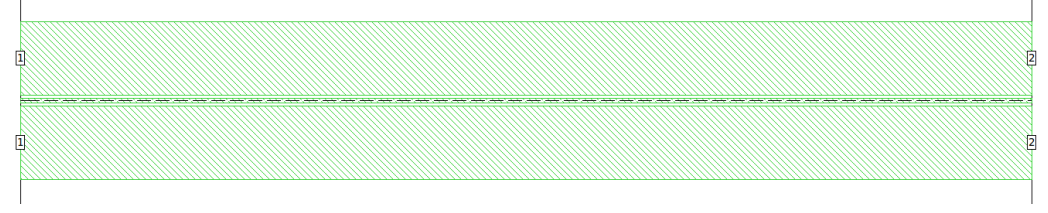
\includegraphics[width=15cm] {Even_cfg1}
\caption{Configuration 1 for even mode simulation}
\label{pic:Even_cfg1}
\end{figure*}

\begin{figure*}[!ht]
\centering
%\captionsetup{singlelinecheck=no, justification = RaggedRight}
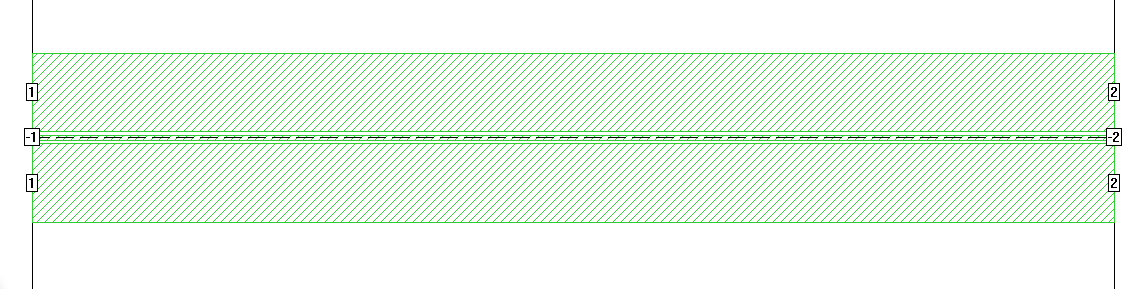
\includegraphics[width=15cm] {Even_cfg2}
\caption{Configuration 2 for even mode simulation}
\label{pic:Even_cfg2}
\end{figure*}


\subsection{Odd mode}

Cfg. 1 for simulating the odd mode is shown in Fig. \ref{pic:Odd_cfg1}. The influence of the box should also be dealt with carefully, for both the central strip and the box are grounded. 

Cfg. 2 (Fig. \ref{pic:Odd_cfg2}) is designed to eliminate the box influence inspired by the Cfg. 2 for the even modes. However, Sonnet produces a warning for this configuration stating that the positive and negative ports should not be shorted together. The corresponding results are also weird. 

Cfg. 3 (Fig. \ref{pic:Odd_cfg3}) is physically similar to Cfg. 1 by utilizing the conductivity of the box to mirror the other half of the waveguide and excite an odd mode. 

\begin{figure*}[!ht]
\centering
%\captionsetup{singlelinecheck=no, justification = RaggedRight}
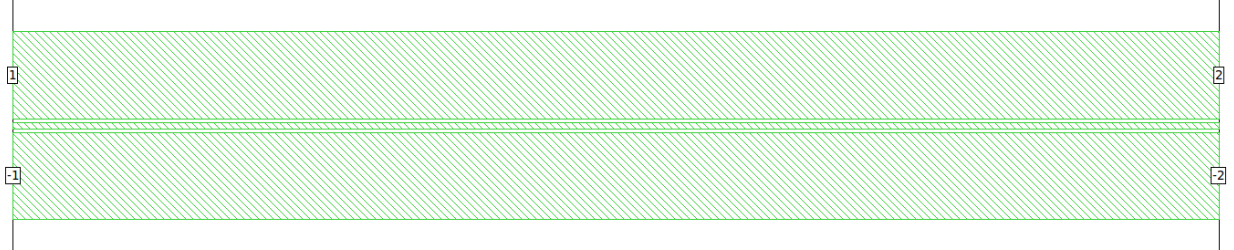
\includegraphics[width=15cm] {Odd_cfg1}
\caption{Configuration 1 for odd mode simulation}
\label{pic:Odd_cfg1}
\end{figure*}

\begin{figure*}[!ht]
\centering
%\captionsetup{singlelinecheck=no, justification = RaggedRight}
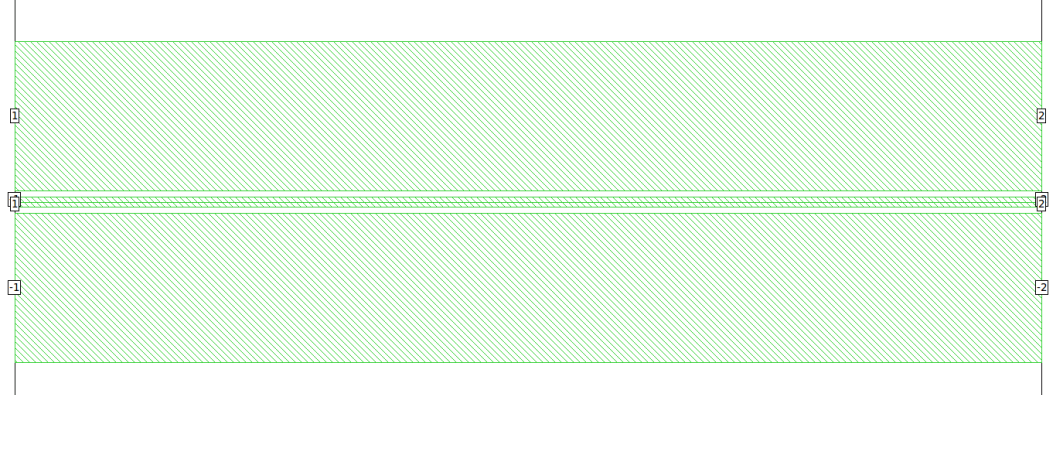
\includegraphics[width=15cm] {Odd_cfg2}
\caption{Configuration 2 for odd mode simulation}
\label{pic:Odd_cfg2}
\end{figure*}

\begin{figure*}[!ht]
\centering
%\captionsetup{singlelinecheck=no, justification = RaggedRight}
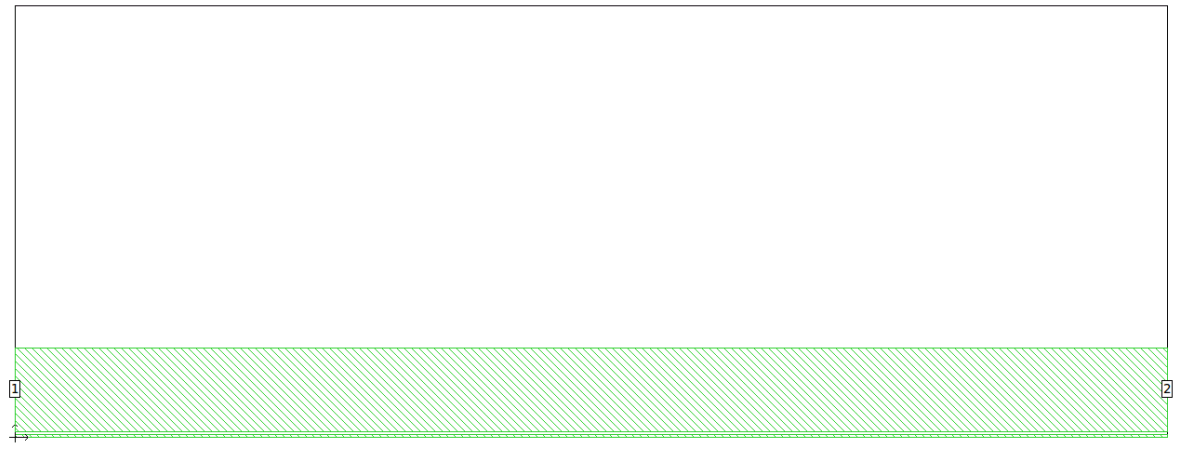
\includegraphics[width=15cm] {Odd_cfg3}
\caption{Configuration 3 for odd mode simulation}
\label{pic:Odd_cfg3}
\end{figure*}

\subsection{Comparison of the results from different configurations} 

\begin{figure*}[!ht]
\centering
%\captionsetup{singlelinecheck=no, justification = RaggedRight}
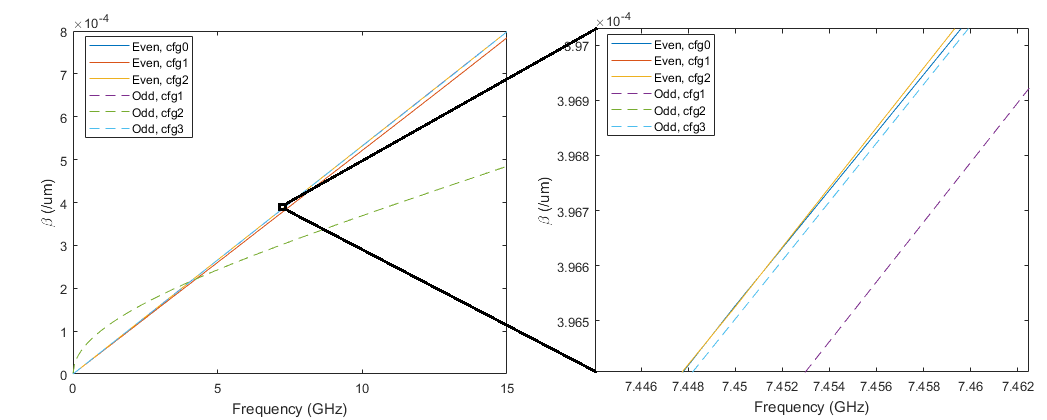
\includegraphics[width=15cm] {Dispersion_all}
\caption{Dispersion relation for the above configurations. The almost overlaid curves are zoomed in.}
\label{pic:Dispersion_all}
\end{figure*}

\begin{figure*}[!ht]
\centering
%\captionsetup{singlelinecheck=no, justification = RaggedRight}
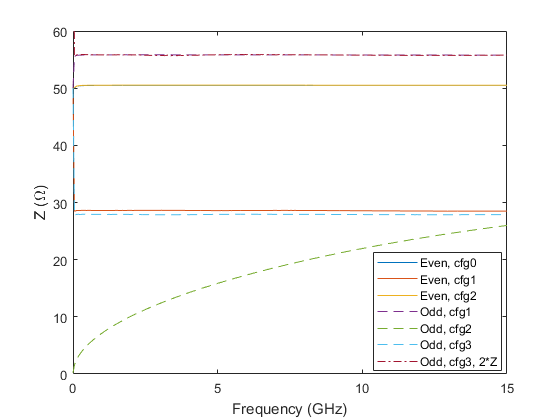
\includegraphics[width=10cm] {Impedance_all}
\caption{Characteristic impedance for the above configurations. Cfg. 0 and Cfg. 2 of the even mode are overlaid. Cfg. 1 and two times the Cfg. 3 of the odd mode are overlaid.}
\label{pic:Dispersion_all}
\end{figure*}

For the even mode, Cfg. 0 and Cfg. 2 give almost the same results but Cfg. 1 deviates a lot especially in the impedance. For the odd mode, Cfg. 2 encounters warnings in Sonnet and the results seem unreliable in characterizing the odd mode. The dispersion curves for Cfg. 1 and 3 are similar and the impedance for Cfg. 1 is almost twice of that for Cfg. 3. It is because Sonnet calculates the differential mode $Z_0$ for Cfg. 1, which is twice the impedance of a single conductor \cite{smolyansky2000characterization}.

\section{Influence of the box size}
Cfg. 1 and 3 to study the odd modes also include the interaction between the panels and the box wall. The changes in the dispersion curve is tiny therefore we use the characteristic impedance as a factor to study the influence of the box size. The dimension parameters used is shown in Fig. \ref{pic:Dimension} and Cfg. 3 is employed to reduce the simulation scale. 

\begin{figure*}[!ht]
\centering
%\captionsetup{singlelinecheck=no, justification = RaggedRight}
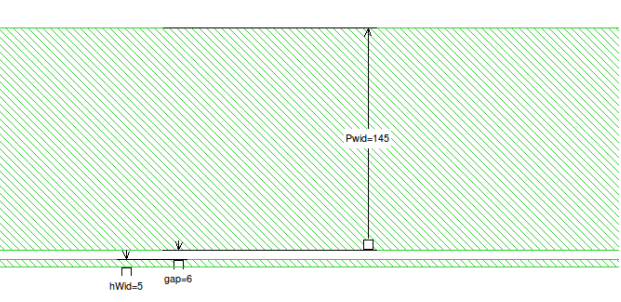
\includegraphics[width=15cm] {Dimension}
\caption{Dimension parameters used in studying the influence of the box size using Cfg. 3 for odd mode.}
\label{pic:Dimension}
\end{figure*}

\begin{figure*}[!ht]
\centering
%\captionsetup{singlelinecheck=no, justification = RaggedRight}
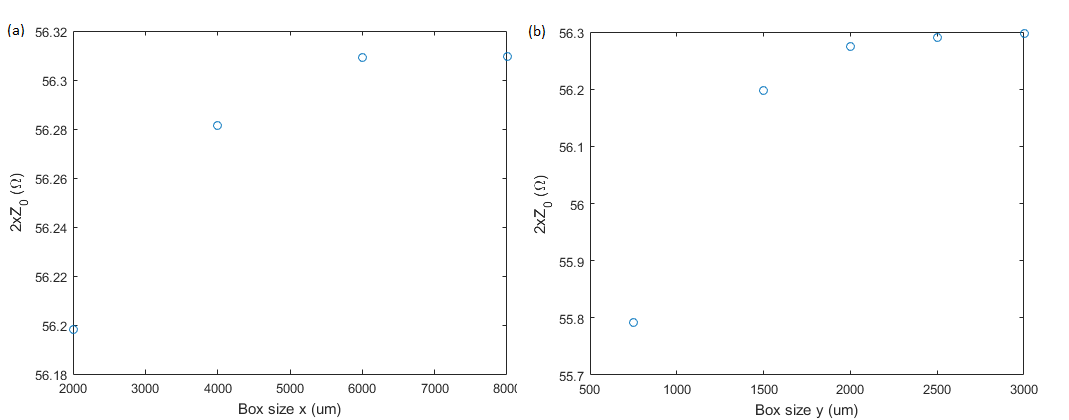
\includegraphics[width=15cm] {Z_bx}
\caption{Characteristic impedance of the waveguide mode with (a) varying box size in the x dimension and fixed box size in the y dimension of 1500 $\upmu$m; (b) varying box size in the y dimension and fixed box size in the x dimension of 2000 $\upmu$m.}
\label{pic:Z_bx}
\end{figure*}

The impedance convergences with a large enough size of the box in both dimensions. 

The impedance of the even mode Cfg. 1 also changes with increasing size of the box, in a even more drastic way  (shown in Table. \ref{tab:even_impd}) because the impedance of the stripline mode is related to the box size. 
%Although the impedance converges when increasing one of the box size parameters, it is actually limited by the other parameter.  

\begin{table}[htbp]
  \centering
  \caption{Characteristic impedance of Cfg. 1 for the even mode}
    \begin{tabular}{lrrrrrrrr}
    Box size (um) & \multicolumn{1}{l}{2k} & \multicolumn{1}{l}{3k} & \multicolumn{1}{l}{4k} & \multicolumn{1}{l}{5k} & \multicolumn{1}{l}{6k} & \multicolumn{1}{l}{7k} & \multicolumn{1}{l}{8k} & \multicolumn{1}{l}{9k} \\
    1k    & 25.97658 &       &       &       &       &       &       &  \\
    2k    & 30.04184 &       &       &       &       &       &       &  \\
    3k    & 31.42586 & 32.38019 & 32.62504 & 32.63833 &       &       &       &  \\
    4k    & 32.02657 &       & 33.6794 & 34.25564 &       &       &       &  \\
    5k    & 32.35488 &       &       &       &       &       &       &  \\
    6k    & 32.56564 &       &       &       &       &       &       &  \\
    7k    &       &       &       &       &       &       &       & 34.63289 \\
    8k    &       &       &       &       &       &       &       &  \\
    9k    &       &       &       &       &       &       &       & 34.94641 \\
    \end{tabular}%
  \label{tab:even_impd}%
\end{table}%

\section{Dimension parameters of the waveguide}

The three tunable dimension parameters of the waveguide is shown in Fig. \ref{pic:Dimension}. The whole geometry is mirrored by the box so that the width of the central strip is actually $2$hWid. For the even mode, the characteristic impedance is determined mainly by hWid and gap (might because there is no current flowing on the outer rim of the panel). But for the odd mode, the width of the panel (Pwid) also matters. 

\begin{figure*}[!ht]
\centering
%\captionsetup{singlelinecheck=no, justification = RaggedRight}
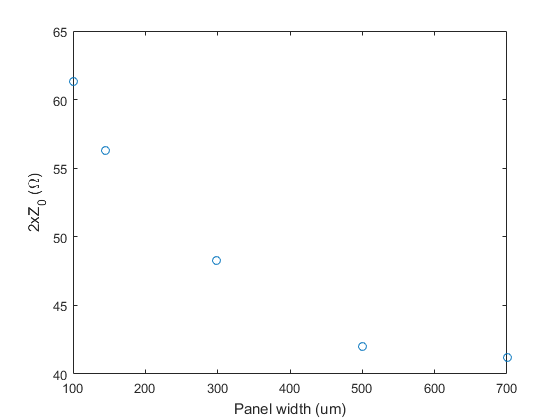
\includegraphics[width=10cm] {Z_panelW}
\caption{Characteristic impedance of the waveguide mode with varying panel width and fixed box size x=2000 $\upmu$m and y=1500 $\upmu$m. Other dimension parameters are fixed and shown in Fig. \ref{pic:Dimension}}
\label{pic:Z_panelW}
\end{figure*}

The impedance is also determined by the width of the central strip and the gap between the central strip and the panel. In the experiment, the impedance of the even mode should be kept to around 50 $\Omega$ in order to match the impedance with the transmission line. With an almost constant impedance for the even mode, the impedance of the corresponding structure for the odd mode is shown in Fig. \ref{pic:Z_cW}.

\begin{figure*}[!ht]
\centering
%\captionsetup{singlelinecheck=no, justification = RaggedRight}
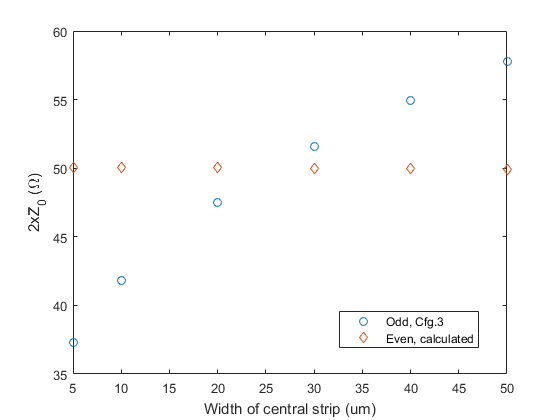
\includegraphics[width=10cm] {Z_cW}
\caption{Characteristic impedance of the waveguide mode with varying panel width and fixed box size x=2000 $\upmu$m and y=1500 $\upmu$m. Other dimension parameters are fixed and shown in Fig. \ref{pic:Dimension}}
\label{pic:Z_cW}
\end{figure*}

\section{Detection of the odd mode}

We have demonstrated above how to excite odd modes in the CPW using Sonnet. The next step would be effectively detecting the odd mode, especially in the case where both the even and odd modes are present. Measuring the $S_{21}$ parameter may help in determining the component of even/odd mode in the total wave. Use the evenly-driven port configuration as the input and the odd port configuration as the output (shown in Fig. \ref{pic:Detection_conf}), and the $S_{21}$ parameter shows the transmitted part of the even mode through the oddly-configured ports, which is typically down to -70 dB or lower. The $S_{21}$ for transmitted odd mode through the odd ports, on the other hand, is nearly 0 dB with matched impedance. Therefore, if a wave with the linear combination of even/odd mode transmits through the odd ports, the $S_{21}$ indicates the portion of odd mode in the total wave. 

\begin{figure*}[!ht]
\centering
%\captionsetup{singlelinecheck=no, justification = RaggedRight}
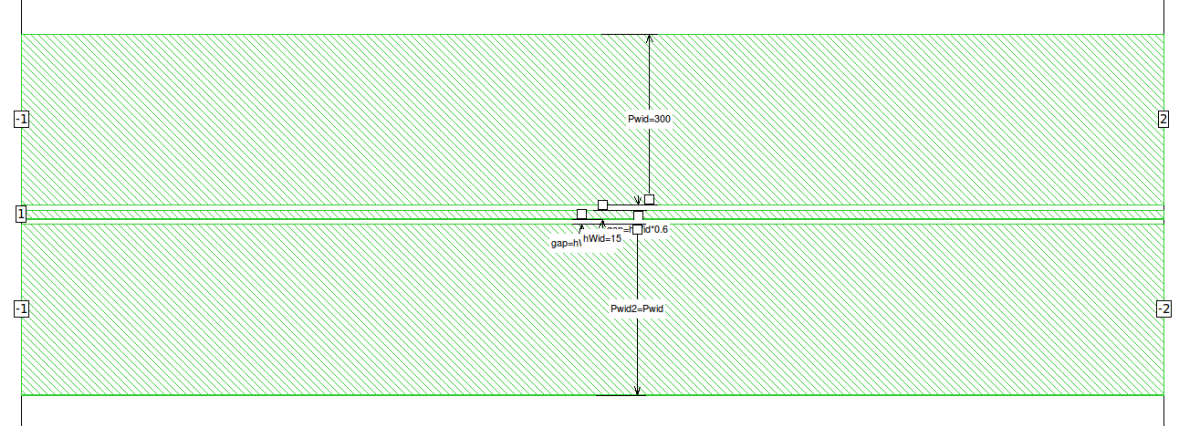
\includegraphics[width=16cm] {Detection_conf}
\caption{Port configuration for detecting the odd mode.}
\label{pic:Detection_conf}
\end{figure*}

Unfortunately, I have not found a way in Sonnet to deterministically excite the combination of even and odd modes with a desired ratio. However, the discontinuity or asymmetry in the CPW, e.g. the unequal width of the ground planes, is known to excite odd mode \cite{ponchak2005excitation}. Here, we use the unequal width of the ground planes in the simulation and compare the detected $S_{21}$ with the results shown in \cite{ponchak2005excitation}. As is shown in Fig. \ref{pic:S_ratioPlaneWidth}, $S_{21}$ drops with the ratio of the ground approaching 1 as expected. We also explored the influence of the propagation distance,  i.e. the length of the waveguide in the simulation, which is shown in Fig. \ref{pic:S_Distance_c}. Our simulation shows a revival of the odd mode that is not reflected from \cite{ponchak2005excitation}.

\begin{figure*}[!ht]
\centering
%\captionsetup{singlelinecheck=no, justification = RaggedRight}
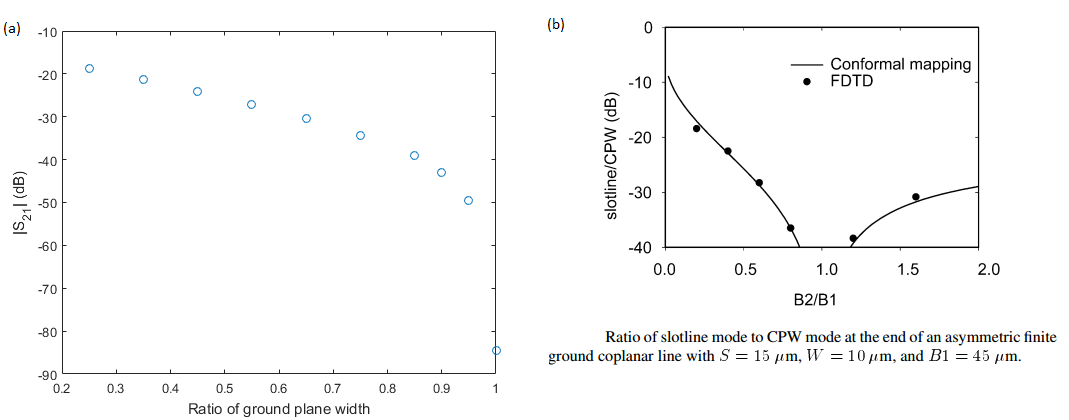
\includegraphics[width=16cm] {S_ratioPlaneWidth_c}
\caption{(a) Simulated $S_{21}$ from Sonnet versus the ratio of the two ground planes with the thinner one fixed at 45 $\upmu$m, the width of the central pin to be 15 $\upmu$m and the gap of 9 $\upmu$m. The length of the waveguide is 12 mm. (b) The result of the same geometry in \cite{ponchak2005excitation}.}
\label{pic:S_ratioPlaneWidth}
\end{figure*}

%\begin{figure*}[!ht]
%\centering
%\captionsetup{singlelinecheck=no, justification = RaggedRight}
%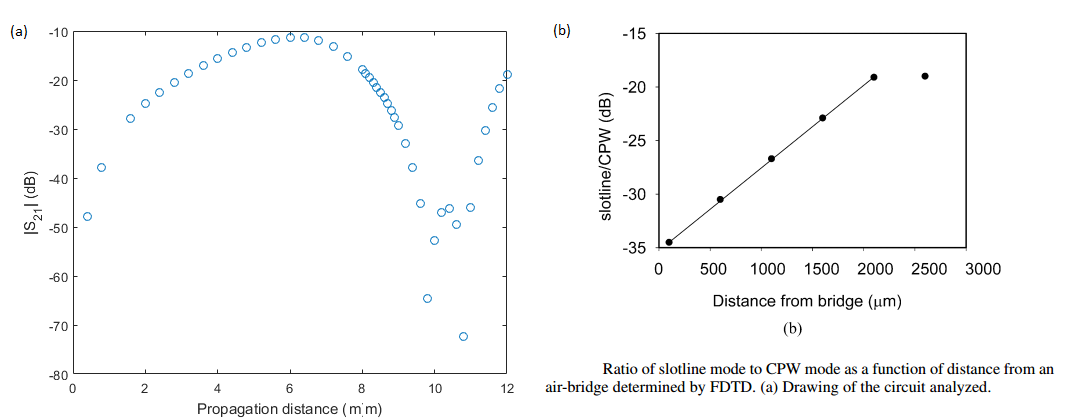
\includegraphics[width=16cm] {S_Distance_c}
%\caption{(a) Simulated $S_{21}$ from Sonnet versus the length of the waveguide. The ratio of the two ground planes is fixed to be 0.25, with the thinner one fixed at 45 $\upmu$m, the width of the central pin to be 15 $\upmu$m and the gap of 9 $\upmu$m. (b) The result of the same geometry in \cite{ponchak2005excitation}.}
%\label{pic:S_Distance_c}
%\end{figure*}

\section{Coupling to the resonator}

Taking a step foward, we simulated the coupling between a resonator (typical quarter wavelength resoantor) to the waveguide even/odd mode, as is shown in Fig. \ref{pic:ResCp_geo}. The box size is 3k by 7k ($\upmu m^2$) and the width of the ground plane is 2k $\upmu$m. Three different coupling methods, inductive, capacitive and directly capacitive coupling (see Fig. \ref{pic:Cpl_cfg}), are compared. In each cases, the coupling strength and intrinsic loss are extracted with different width of the central trace (see Fig. \ref{pic:tInduc_ke} to \ref{pic:eCap_ki}). For all of the coupling methods, the coupling to the odd mode is stronger than that to the even mode, which is believed to originate from the current distribution of the two modes. The current of even mode is highly concentrated on the central trace while the current of odd mode is more spread out in the ground plane, indicating a larger overlap with the resonator embedded in the ground plane (Fig. \ref{pic:Even_waveguide}). Increasing width of the central trace, the external coupling strength increases for the even mode but decreases for the odd mode. 

\begin{figure*}[!ht]
\centering
%\captionsetup{singlelinecheck=no, justification = RaggedRight}
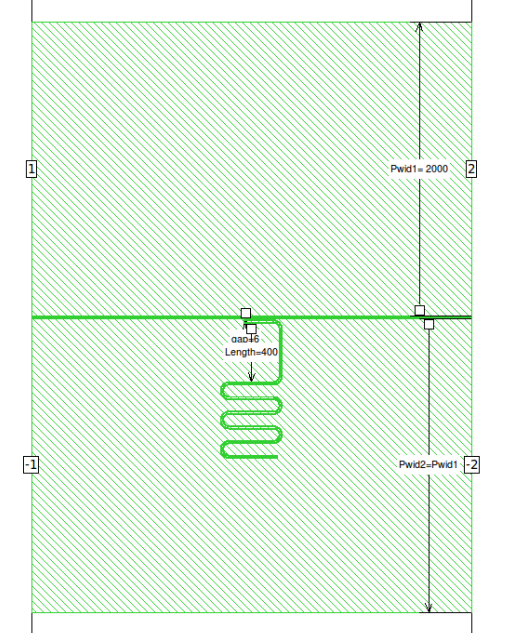
\includegraphics[width=10cm] {ResCp_geo}
\caption{The geometry used to simulate the coupling between the resonator and the waveguide}
\label{pic:ResCp_geo}
\end{figure*}

\begin{figure*}[!ht]
\centering
%\captionsetup{singlelinecheck=no, justification = RaggedRight}
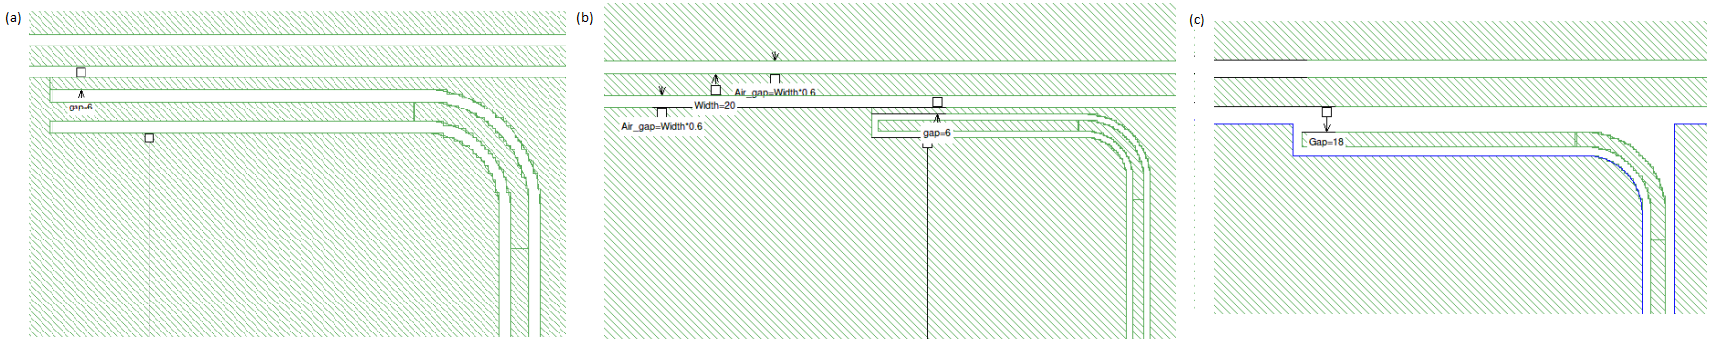
\includegraphics[width=16cm] {Cpl_cfg}
\caption{Three different coupling schemes between the resonator and the waveguide, and the definition of the geometric parameters. (a) Inductive coupling; (b) Capacitive coupling; (c) Direct capacitive coupling. }
\label{pic:Cpl_cfg}
\end{figure*}

%\begin{figure*}[!ht]
%\centering
%\captionsetup{singlelinecheck=no, justification = RaggedRight}
%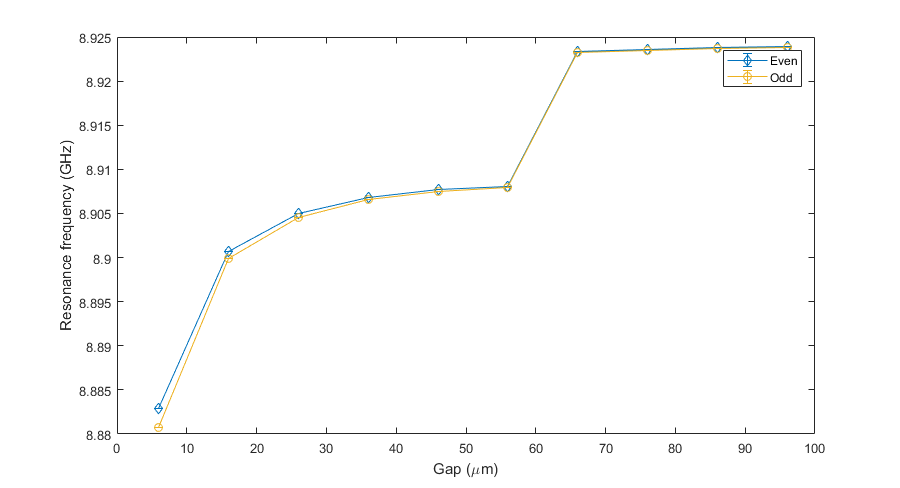
\includegraphics[width=15cm] {Rfreq_gap}
%\caption{Resonance frequency versus the gap between the resonator and the waveguide. The error bars (and the next two figures) represent 99\% confidence interval.}
%\label{pic:Rfreq_gap}
%\end{figure*}

\begin{figure*}[!ht]
\centering
%\captionsetup{singlelinecheck=no, justification = RaggedRight}
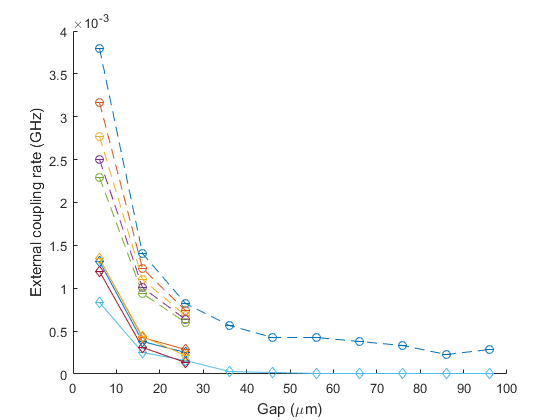
\includegraphics[width=12cm] {tInduc_ke}
\caption{External coupling rate versus the gap between the inductively coupled resonator and the waveguide. The error bars (and the next five figures) represent 99\% confidence interval. The coupling to the odd mode of the waveguide is shown in circles connected by dashed line and the results for even mode are shown in diamond connected by solid lines. For the odd mode, the external coupling rate decreases as the width of the central pin increases (W = 10, 20, 30, 40, 50 $\upmu$m). For the odd mode, the external coupling rate increases as the width of the central pin increases (W = 10, 20, 30, 40, 50 $\upmu$m). The notation of the symbols, colors and lineshape is kept the same for the next five figures.}
\label{pic:tInduc_ke}
\end{figure*}

\begin{figure*}[!ht]
\centering
%\captionsetup{singlelinecheck=no, justification = RaggedRight}
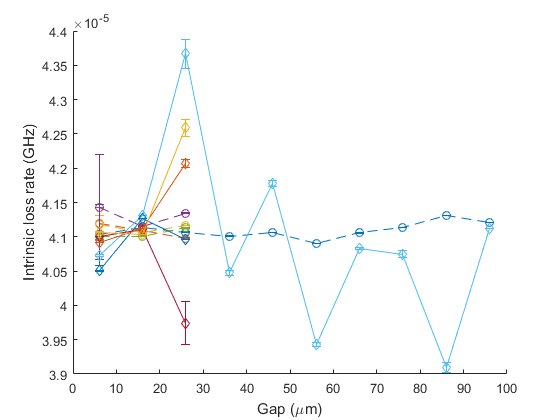
\includegraphics[width=12cm] {tInduc_ki}
\caption{Intrinsic loss rate versus the gap between the inductively coupled resonator and the waveguide. }
\label{pic:tInduc_ki}
\end{figure*}

\begin{figure*}[!ht]
\centering
%\captionsetup{singlelinecheck=no, justification = RaggedRight}
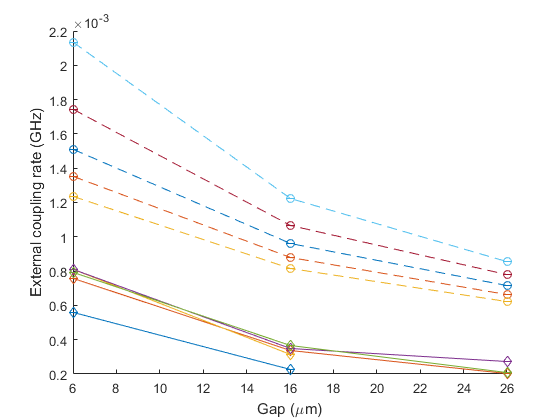
\includegraphics[width=12cm] {tCap_ke}
\caption{External coupling rate versus the gap between the capacitively coupled resonator and the waveguide.}
\label{pic:tCap_ke}
\end{figure*}

\begin{figure*}[!ht]
\centering
%\captionsetup{singlelinecheck=no, justification = RaggedRight}
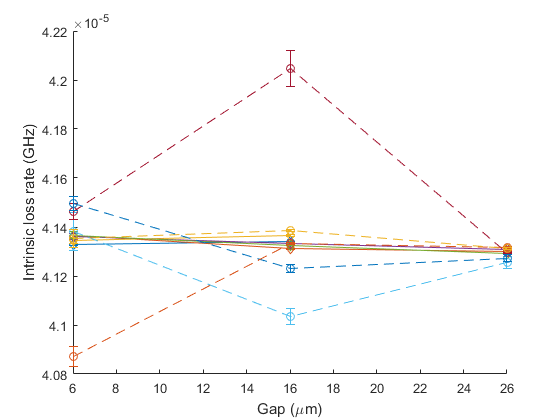
\includegraphics[width=12cm] {tCap_ki}
\caption{Intrinsic loss rate versus the gap between the capacitively coupled resonator and the waveguide.}
\label{pic:tCap_ki}
\end{figure*}

\begin{figure*}[!ht]
\centering
%\captionsetup{singlelinecheck=no, justification = RaggedRight}
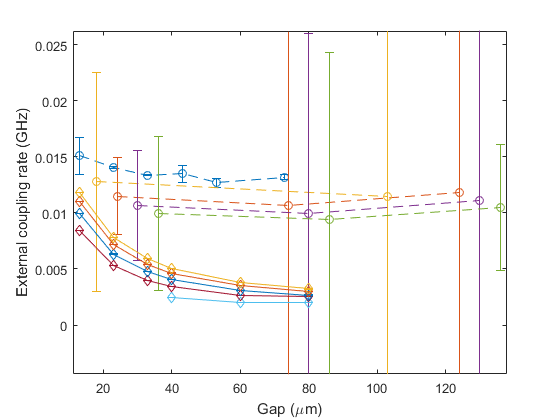
\includegraphics[width=12cm] {eCap_ke}
\caption{External coupling rate versus the gap between the directly-capacitively coupled resonator and the waveguide.}
\label{pic:eCap_ke}
\end{figure*}

\begin{figure*}[!ht]
\centering
%\captionsetup{singlelinecheck=no, justification = RaggedRight}
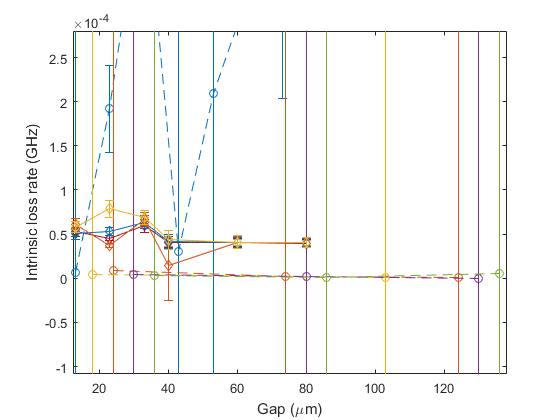
\includegraphics[width=12cm] {eCap_ki}
\caption{Intrinsic loss coupling rate versus the gap between the directly-capacitively coupled resonator and the waveguide.}
\label{pic:eCap_ki}
\end{figure*}

\begin{figure*}[!ht]
\centering
%\captionsetup{singlelinecheck=no, justification = RaggedRight}
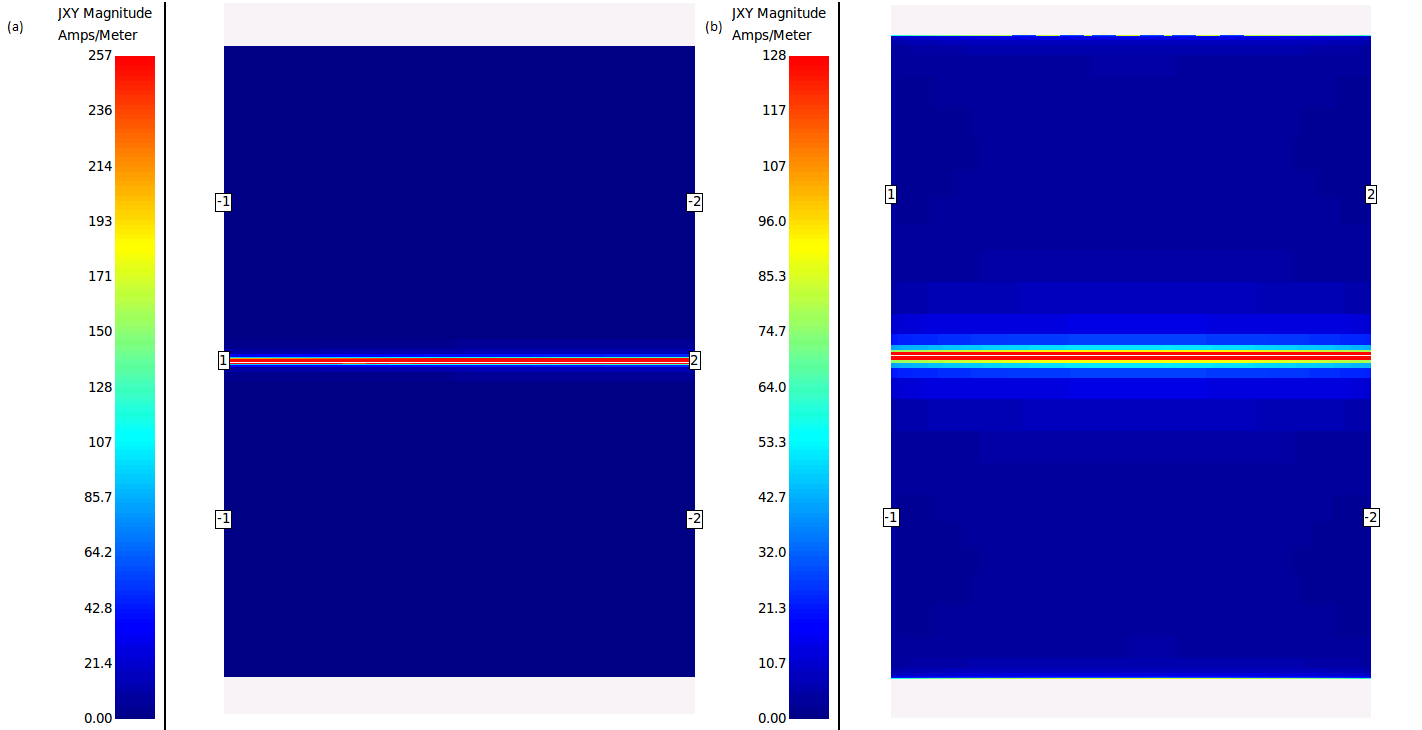
\includegraphics[width=16cm] {Even_waveguide}
\caption{The current view of waveguide excited by (a) even and (b) odd ports configuration}
\label{pic:Even_waveguide}
\end{figure*}

Similar to the detection of the odd mode in the waveguide, a hybrid port configuration is also incorporated in testing the coupling of the resonator to the waveguide mode. On the resonance, there is a large portion of even mode converted to the odd mode through the resonator (Fig. \ref{pic:Hybd_geo}). Note that, the boundary reflective for one of the mode, so the scattering parameter is a result of both the coupling between even/odd mode through the resonator and the reflection and interference at the port.

\begin{figure*}[!ht]
\centering
%\captionsetup{singlelinecheck=no, justification = RaggedRight}
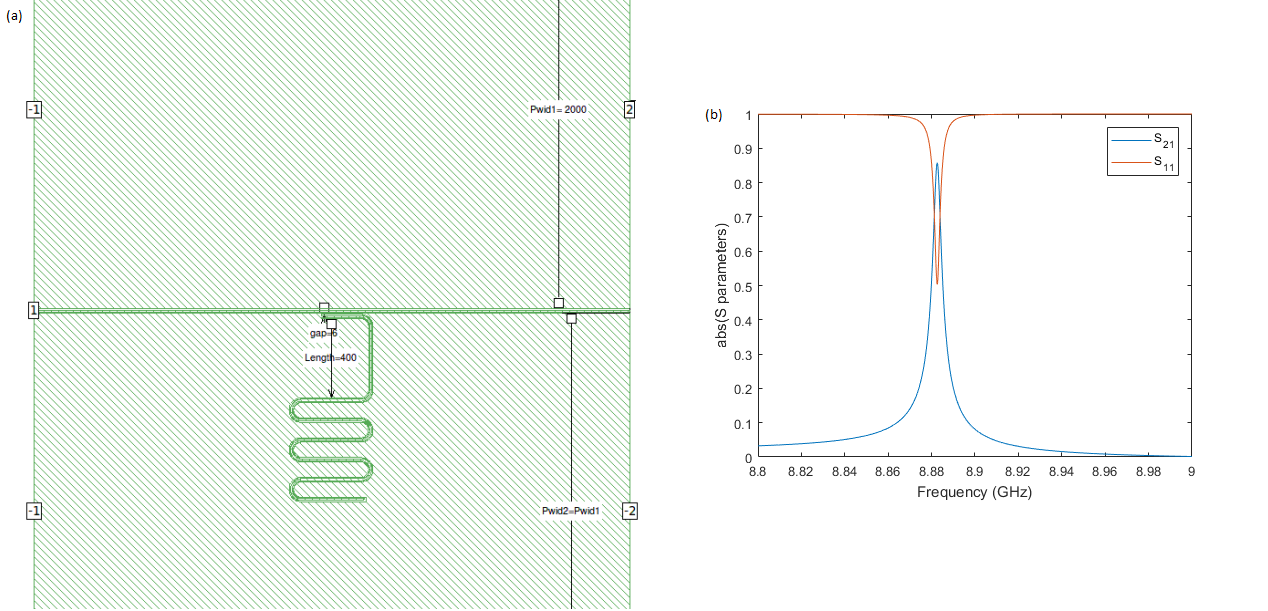
\includegraphics[width=16cm] {Hybd_geo}
\caption{(a) Hybrid port configuration for waveguide inductively coupling with the resonator and the corresponding scattering parameters $S_{21}$ and (b) $S_{11}$ at gap=6 $\upmu$m.}
\label{pic:Hybd_geo}
\end{figure*}

%\begin{figure*}[!ht]
%\centering
%%\captionsetup{singlelinecheck=no, justification = RaggedRight}
%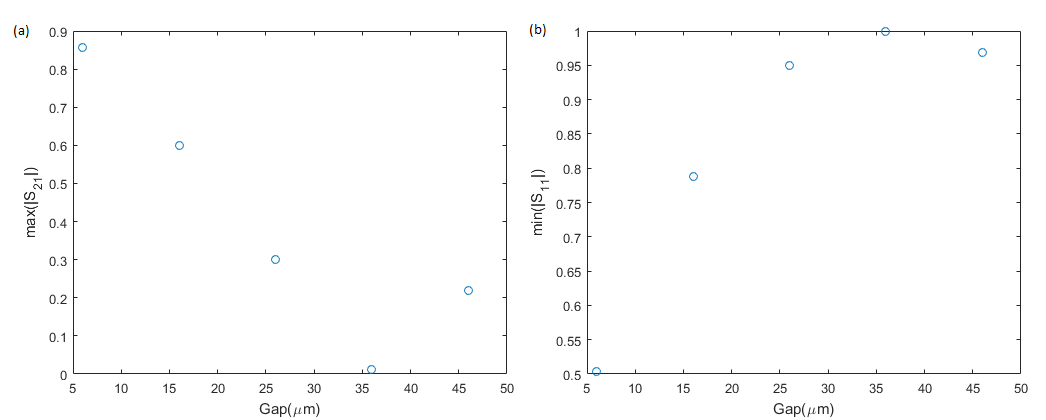
\includegraphics[width=16cm] {S21_gap_hyb}
%\caption{Scattering parameters (a) $S_{21}$ and (b) $S_{11}$ versus the gap with port 1 using even Cfg. 2 and port 2 using odd Cfg. 1}
%\label{pic:S21_gap_hyb}
%\end{figure*}

\section{Coupling to a qubit}

The coupling between a qubit and the waveguide even/odd mode is also simulated. Particularly, we simulated and compared the  two different configurations of qubit (namely, Xmon and transmon) in order to see the influence of different geometries (Fig. \ref{pic:Lo_Xtransmon}).

 \begin{figure*}[!ht]
\centering
%\captionsetup{singlelinecheck=no, justification = RaggedRight}
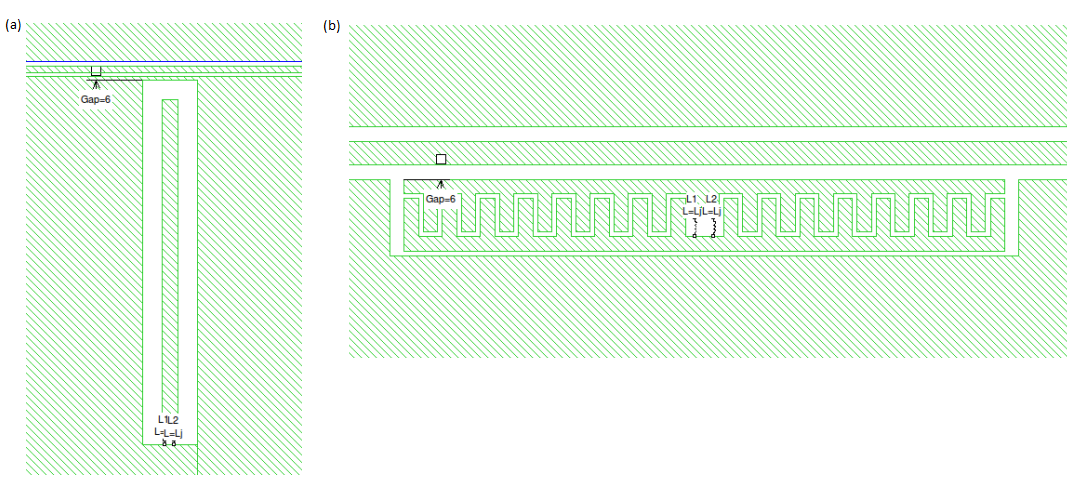
\includegraphics[width=16cm] {Lo_Xtransmon}
\caption{Geometry of coupling between (a) Xmon and (b) transmon to the waveguide. The resonance frequencies of the two qubit are set to the same at 8.8 GHz.}
\label{pic:Lo_Xtransmon}
\end{figure*}

\begin{figure*}[!ht]
\centering
%\captionsetup{singlelinecheck=no, justification = RaggedRight}
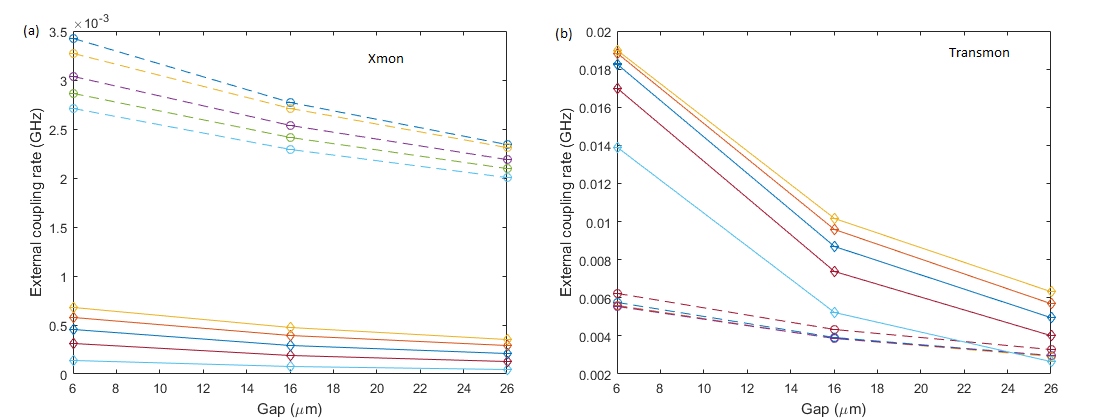
\includegraphics[width=16cm] {ke_Xmon}
\caption{External coupling rate versus the gap between (a) Xmon (b) transmon and the waveguide. The error bars (and the next figure) represent 99\% confidence interval. The coupling to the odd mode of the waveguide is shown in circles connected by dashed line and the results for even mode are shown in diamond connected by solid lines. For the odd mode, the external coupling rate decreases as the width of the central pin increases (W = 10, 20, 30, 40, 50 $\upmu$m). For the odd mode, the external coupling rate increases as the width of the central pin increases (W = 10, 20, 30, 40, 50 $\upmu$m). The notation of the symbols, colors and lineshape is kept the same for the next figure.}
\label{pic:ke_Xmon}
\end{figure*}

\begin{figure*}[!ht]
\centering
%\captionsetup{singlelinecheck=no, justification = RaggedRight}
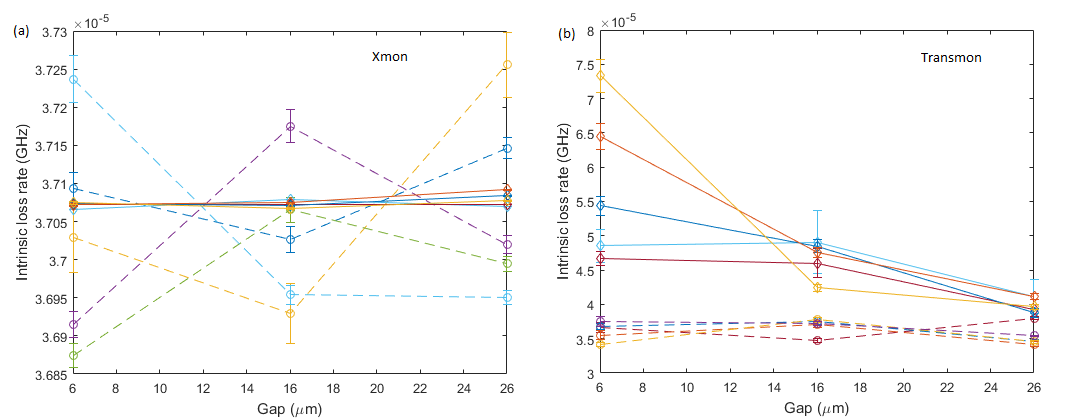
\includegraphics[width=16cm] {ki_Xmon}
\caption{Intrinsic loss coupling rate versus the gap between (a) Xmon (b) transmon and the waveguide.}
\label{pic:ki_Xmon}
\end{figure*}

The external coupling rate and the intrinsic loss rate of the two kinds of qubit coupling with the waveguide is shown in Fig. \ref{pic:ke_Xmon} and \ref{pic:ki_Xmon}. The coupling between the Xmon and the waveguide is similar to that of a resonator to the waveguide. For transmon, the coupling to the even mode is more than two times larger than that to the odd mode. 



\bibliography{ref}




\end{document}
